\subsection*{Magnetische Feldstärke H}
    \begin{minipage}{0.59\linewidth}
        \begin{itemize}
            \item Stromdurchflossene Leiter bauen magnetisches Feld auf
            \item Rechte-Hand-Regel
        \end{itemize}
        \centering \underline{\textbf{Spule}}\\
        \begin{minipage}{0.44\linewidth}
            \mathbox{\left| \vec{H} \right| = I \frac{n}{l}}
        \end{minipage}
%
        \begin{minipage}{0.54\linewidth}
            \begin{scriptsize}
                \begin{empheq}{align*}
                    H &= \text{Magnetische Feldstärke}\\
                    I &= \text{Stromstärke}\\
                    n &= \text{Windungen der Spule}\\
                    l &= \text{Länge der Spule}\\
                \end{empheq}
            \end{scriptsize}
        \end{minipage}
    \end{minipage}
%
    \begin{minipage}{0.39\linewidth}
        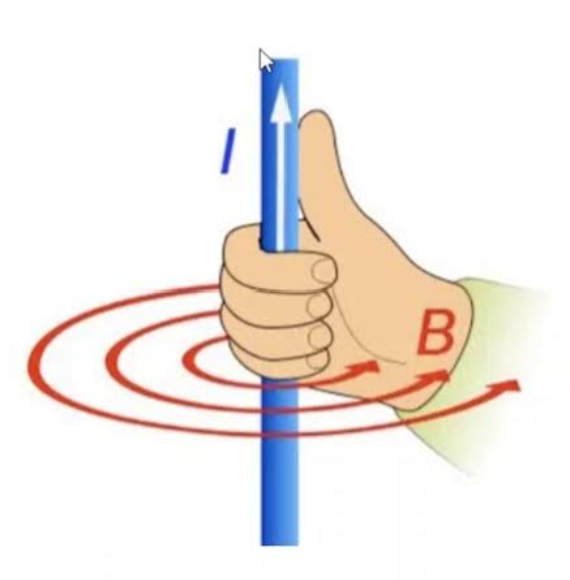
\includegraphics[width = \linewidth]{src/images/rechte_hand_magnetismus.png}
    \end{minipage}
    